%%		Solutions to Shifrin's Differential Geometry
%%		Chapter One: Curves , Section One: Examples
\documentclass[Shifrin_Solutions_Spring_2018]{subfiles}
\begin{document}


\section{Examples, Arclength Parameterization}

\begin{exercise}
Parametrize the unit circle (less the point $(-1,0)$)  by the signed length $t$
of the vertical line segment joining the origin to the chord from $(-1,0)$ to
the point on the circle.
\end{exercise}

\begin{proof}[Solution]
Note that $t \in (-\infty, \infty)$ is the slope of the line through
$P = (-1,0)$ and $Q = (0,t)$. Using the point-slope form of a line through $P$,
our generic point $(x,y)$ must satisfy this linear equation:
\[
y = t ( x+1).
\]
Because our point sits at the intersection of this line with the circle
$x^2  + y^2 = 1$, the numbers $x$ and $y$ are a simultaneous
solution of these two equations\dots So we substitute the first into the second
to find:
\[
1 = x^2 + y^2 = x^2 + [t(x+1)]^2 = x^2 + t^2x^2 + 2t^2x + t^2.
\]
We rearrange this into a quadratic equation in $x$ whose coefficients depend
upon $t$,
\[
(1+t^2) x^2 + (2t^2) x + (t^2 - 1) = 0,
\]
and use the quadratic formula to find the roots. After some simplifying, we
obtain
\[
x = \dfrac{-t^2 \pm \sqrt{1}}{1+t^2}.
\]
Choosing the negative branch of the square root leads to $x=-1$, which means
that we get the point $P$. This is good! The point $P$ is a point of
intersection of the line with the circle, but we want the \emph{other}
intersection. To find the interesting point, we choose the positive
branch of the square root and obtain
\[
x = \dfrac{1-t^2}{1+t^2}.
\]
We go back to the equation of the circle to find the expression for $y$, which
becomes
\[
y =\pm \dfrac{ 2|t|}{1+t^2}.
\]
It is clear from our diagram that $y$ and $t$ have the same sign, so our final
parametrization is
\[
x = \dfrac{1-t^2}{1+t^2}, \qquad y = \dfrac{ 2t}{1+t^2}, \quad \mbox{ for } t
\in (-\infty, \infty) .
\]
\end{proof}

\clearpage

%%%%%%%%%%%%%%%%%%%%%%%%%%%%%%%%%%%%%%%%%%%%

\begin{exercise}
Consider the helix $\alpha(t) = ( a \cos t , a \sin t , b t )$. Calculate
$\alpha'(t)$,
$||\alpha'(t)||$ and reparametrize $\alpha$ by arclength.
\end{exercise}

\begin{proof}[Solution] We compute directly
\[
\alpha'(t) = ( - a \sin t, a \cos t , b)
\]
\[
||\alpha'(t)|| = [ (-a\sin t)^2 + (a \cos t)^2 + b^2]^{1/2} = [a^2+b^2]^{1/2}
\]
So $\alpha$ has constant speed. This makes reparameterizing a snap. We use the
function
\[
t = h(s) = \dfrac{s}{\sqrt{a^2 + b^2 \ }}.
\]
Now $\beta(s) = \alpha \circ h(s) = \alpha(h(s))$ has $||\beta'(s)|| =
||\alpha'(t)||\cdot |h'(s)| = 1$.
We conclude that an arclength reparameterization of the curve is
\[
\beta(s) = \left( a \cos \left(\dfrac{s}{\sqrt{a^2 + b^2 \ }}\right) , a
\sin\left( \dfrac{s}{\sqrt{a^2 + b^2 \ }}\right) , \dfrac{b \cdot s}{\sqrt{a^2
+ b^2 \ }} \right).
\]
\end{proof}

\begin{figure}[h]
\centering
\subfloat[Exercise 1.1.2: A Helix with $a=7$,
$b=3$]{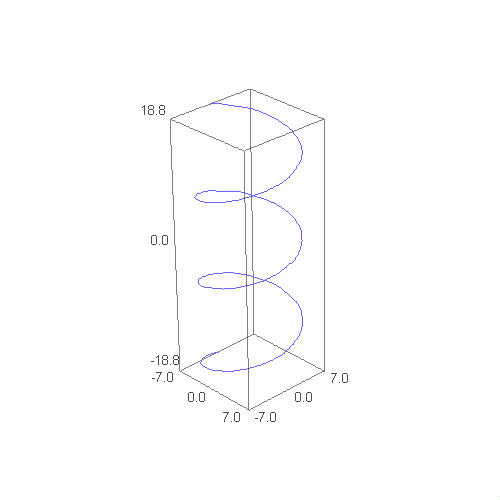
\includegraphics[width=0.48\textwidth]{picturebook/ch1sec1/ex1-1-2}}
  \subfloat[Exercise 1.1.3: A Circle]{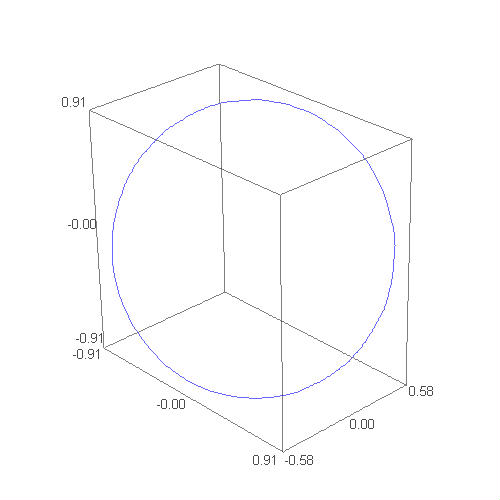
\includegraphics[width=0.48\textwidth]{picturebook/ch1sec1/ex1-1-3}}
  \caption{The curves from Exercises 1.1.2 and 1.1.3}
\end{figure}


\clearpage

%%%%%%%%%%%%%%%%%%%%%%%%%%%%%%%%%%%%%%%%%%%%


\begin{exercise} Let
$\alpha (t) = \left( \dfrac{1}{\sqrt{3}} \cos t + \dfrac{1}{\sqrt{2}}\sin t , 
\dfrac{1}{\sqrt{3}}\cos t , \dfrac{1}{\sqrt{3}}\cos t - \dfrac{1}{\sqrt{2}}\sin t \right)$.
Calculate $\alpha'(t)$, $|| \alpha'(t)||$, and reparameterize $\alpha$ by arclength.
\end{exercise}

\begin{proof}[Solution]
We compute
\[
\alpha'(t) = \left(  -\dfrac{1}{\sqrt{3}}\sin t + \dfrac{1}{\sqrt{2}}\cos t ,
- \dfrac{1}{\sqrt{3}} \sin t ,
-\dfrac{1}{\sqrt{3}}\sin t - \dfrac{1}{\sqrt{2}}\cos t
\right) .
\]
So then
\[
||\alpha'(t)||^2 = \left( -\dfrac{1}{\sqrt{3}}\sin t + \dfrac{1}{\sqrt{2}}\cos t 
\right)^2 + \left( - \dfrac{1}{\sqrt{3}} \sin t \right)^2 + 
\left( -\dfrac{1}{\sqrt{3}}\sin t - \dfrac{1}{\sqrt{2}}\cos t \right)^2 = 1 .
\]
So we see that $\alpha$ is already a unit speed curve, and no reparametrization is necessary.
\end{proof}

\vspace{.5in}

%%%%%%%%%%%%%%%%%%%%%%%%%%%%%%%%%%%%%%%%%%%%


\begin{exercise}
Parametrize the graph $y=f(x)$, $a\leq x \leq b$, and show that its arclength is given 
by the traditional formula
\[
\text{length} = \int_a^b \sqrt{1+(f'(x))^2\,}\, dx .
\]
\end{exercise}

\begin{proof}[Solution]
We parameterize the graph by
\[
x = t, \quad y = f(t), \quad a \leq t \leq b .
\]
That is,
\[
\alpha(t) = \left( t, f(t) \right).
\]
Then
\[
\alpha'(t) = \left( 1, f'(t) \right),
\]
and
\[||\alpha'(t)|| = \sqrt{1 + (f'(t))^2\,} .
\]
So the claim follows directly from the definition of arclength.
\end{proof}

\clearpage

%%%%%%%%%%%%%%%%%%%%%%%%%%%%%%%%%%%%%%%%%%%%


\begin{exercise}{$\ $}
\begin{itemize}
\item[a.] Show that the arclength of the catenary $\alpha(t) = (t, \cosh t)$ for 
$0\leq t\leq b$ is $\sinh b$.

\item[b.] Reparametrize the catenary by arclength.
\end{itemize}
\end{exercise}

\begin{proof}[Solution]
We compute the arclength directly using the Fundamental Theorem of Calculus as
\[
\text{length} = \int_0^b \sqrt{1 + \sinh^2 t } \, dt = \int_0^b \cosh t \, dt = \sinh b .
\]
So, now we must invert the function 
$s = \sinh t = \dfrac{1}{2} \left( e^t - e^{-t}\right)$. 
We first massage it into a form which is reminiscent of a quadratic polynomial
\begin{align*}
2s & = e^t - e^{-t} \\
2se^t &= e^{2t} - 1 \\
(e^t)^2  - 2 s& (e^t) - 1 = 0
\end{align*}
Then, we use the quadratic formula to deduce that
\[
e^t  = \dfrac{2s \pm \sqrt{4s^2 - 4(1)(-1)} }{2(1)} = s \pm \sqrt{s^2+1} .
\]
We choose the positive branch to fit our situation, and then invert the exponential.
\[ t = h(s) = \ln(  s + \sqrt{s^2+1} ) . \]
So, after some computation, we see that the reparametrization of $\alpha$ by 
arclength is the curve
\[
\beta(s) = \alpha\circ h(s) = \left(  s + \sqrt{s^2+1}\, , \,
\dfrac{s^2+1 + s\sqrt{s^2+1 } }{ s + \sqrt{s^2+1 } }\, \right).
\]
\end{proof}

\begin{figure}[h!]
\centering
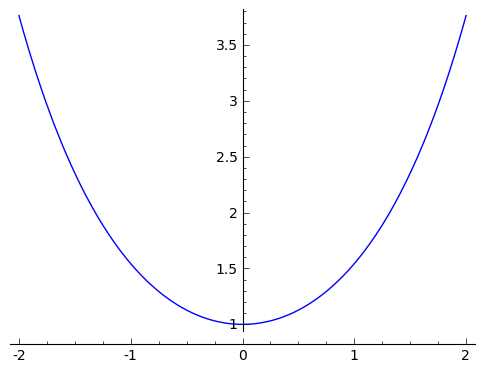
\includegraphics[width=0.5\textwidth]{picturebook/ch1sec1/ex1-1-5}
\caption{Exercise 1.1.5: The Catenary}
\end{figure}



\clearpage

%%%%%%%%%%%%%%%%%%%%%%%%%%%%%%%%%%%%%%%%%%%%


\begin{exercise}
Consider the curve $\alpha(t) = \left( e^t , e^{-t} , \sqrt{2\,} t \right)$. 
Calculate $\alpha'(t)$, $||\alpha'(t)||,$ and reparametrize $\alpha$ by arclength, 
starting at $t=0$.
\end{exercise}

\begin{proof}[Solution]
First we do the computations.
\begin{align*}
\alpha'(t) & = \left( e^t , -e^{-t} , \sqrt{2} \right) , \\
||\alpha'(t) || & =\sqrt{ e^{2t} + e^{-2t} + 2} \\
& = \sqrt{( e^t + e^{-t}  )^2} \\
& = e^t + e^{-t}
\end{align*}
Thus,
\[
s = \int_0^t (e^u + e^{-u} ) \, du = \int_0^t 2\cosh u \, du = 2 \sinh t.
\]
Using a little of what we did in the last exercise, we see that
\[
t = h(s) = \ln\left( \dfrac{s}{2} + \sqrt{\left(\dfrac{s}{2}\right)^2 + 1 } \right)
\]
is our ``time change'' function, and our reparametrized curve is
\[
\beta(s) = \alpha\circ h(s) = \left(
 \dfrac{s}{2} + \sqrt{\left(\dfrac{s}{2}\right)^2 + 1 } \, ,
\left( \dfrac{s}{2} + \sqrt{\left(\dfrac{s}{2}\right)^2 + 1 }\right)^{-1} \, ,
\sqrt{2}\ln\left(\dfrac{s}{2} + \sqrt{ \left(\dfrac{s}{2}\right)^2+1 } \right) \right) .
\]

Note that the middle coordinate is
\[
\left(\dfrac{s}{2} + \sqrt{\left(\dfrac{s}{2}\right)^2 + 1 }\right)^{-1} =  
- \dfrac{s}{2} + \sqrt{\left(\dfrac{s}{2}\right)^2 + 1\, }  .
\]

\end{proof}

\begin{figure}[h!]
\centering
\subfloat[Ex 6: Generalized Helix]{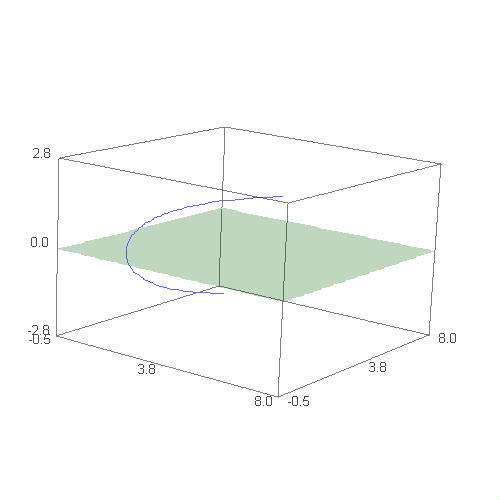
\includegraphics[width=0.4\textwidth]{picturebook/ch1sec1/ex1-1-6-1}}
\subfloat[Ex 6: Another View]{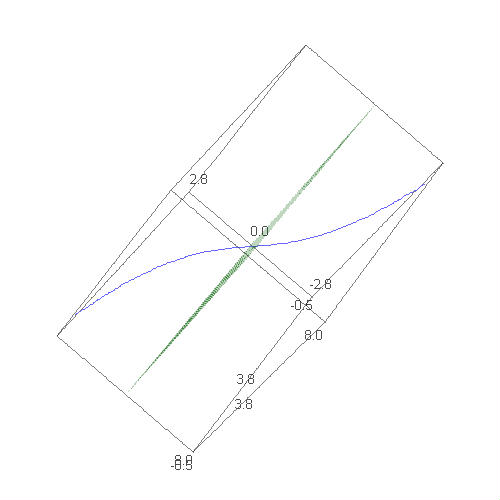
\includegraphics[width=0.4\textwidth]{picturebook/ch1sec1/ex1-1-6-2}}
\caption{Figures for Exercise 1.1.6}
\end{figure}


\clearpage

%%%%%%%%%%%%%%%%%%%%%%%%%%%%%%%%%%%%%%%%%%%%


\begin{exercise}
Find the arclength of the tractrix starting at $(0,1)$ and proceeding to an arbitrary point.
\end{exercise}

\begin{proof}[Solution]
Our curve is
\[
\alpha(\theta) = \left( \cos \theta + \ln \tan( \theta/2 )\, , \sin\theta \right) , 
\qquad \pi/2 \leq \theta < \pi .
\]
We compute in the standard way.
\[
\alpha'(\theta) = \left( -\sin\theta + \dfrac{\sec^2(\theta/2)}{2\tan(\theta/2)}\, , 
\cos\theta \right) .
\]
So, after a massive simplification,
\[
\begin{split}
||\alpha'(t) ||  & = \sqrt{  \sin^2\theta  -\dfrac{\sec^2(\theta/2)\sin(\theta)}{\tan(\theta/2)} 
+ \dfrac{1}{4}\dfrac{\sec^4(\theta/2)}{\tan^2(\theta/2)} + \cos^2\theta   } \\
& = \ldots \\
& =   \dfrac{\cos \theta}{\sin\theta}
\end{split}
\]
Now we can compute the arclength:
\[
\text{length} = \int_{\pi/2}^{\theta} \dfrac{\cos u}{\sin u} \, du = \ln \sin \theta .
\]
\end{proof}

\begin{figure}[h]
\centering
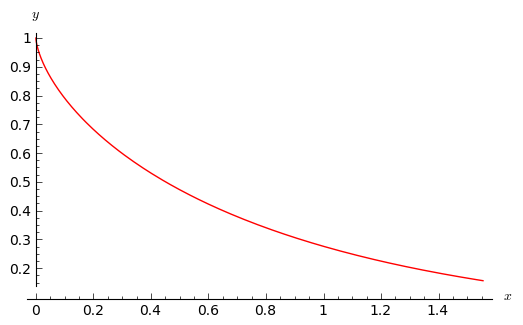
\includegraphics[width=.75\textwidth]{picturebook/ch1sec1/ex1-1-7}
\caption{Exercise 1.1.7: The Tractrix}
\end{figure}

\clearpage

%%%%%%%%%%%%%%%%%%%%%%%%%%%%%%%%%%%%%%%%%%%%


\begin{exercise}
Let $P, Q \in \mathbb{R}^3$ and let $\alpha: [a,b] \rightarrow \mathbb{R}^3$ 
be any parameterized curve with $\alpha(a) = P$ and $\alpha(b) = Q$. Let 
$v= Q-P$. Prove that $\text{length}(\alpha) \geq ||v||$, so that the line 
segment from $P$ to $Q$ gives the shortest possible path.
\end{exercise}

\begin{proof}[Solution]
Note that
\[
\dfrac{d}{dt}\left( \alpha(t)\cdot v \right) = \alpha'(t)\cdot v ,
\]
so by the Fundamental Theorem of Calculus,
\[
\begin{split}
||v||^2 & = v \cdot v \\
  & =  \alpha(b)\cdot v - \alpha(a) \cdot v  \\
	& =  \int_a^b \dfrac{d}{dt}\left( \alpha(t)\cdot v \right) \, dt \\
  & = \int_a^b \alpha'(t)\cdot v \, dt \\
\end{split}
\]
Now recall the Cauchy-Schwarz inequality for vectors in $\mathbb{R}^3$ is
\[
| u \cdot w | \leq ||u||\, ||w||.
\]
If we apply this to the integrand with $u = \alpha(t)$ and $w=v$, we see that
\[
\begin{split}
||v||^2 & = \int_a^b \alpha'(t) \cdot v \, dt \\
	& \leq \int_a^b ||\alpha'(t)|| \, ||v||\, dt \\
  & = ||v|| \int_a^b ||\alpha'(t)||\, dt
\end{split}
\]
Now we divide through by the number $||v||$ to get the result.
\end{proof}

\clearpage

%%%%%%%%%%%%%%%%%%%%%%%%%%%%%%%%%%%%%%%%%%%%


\begin{exercise}
Consider a uniform cable with density $\delta$ hanging in equilibrium. The 
tension forces $T(x + \Delta x)$, $-T(x)$, and the weight of the piece of cable 
lying over $[x,x+\Delta x]$ all balance. If the bottom of the cable is at $x=0$, 
$T_0$ is the magnitude of the tension there, and the cable is the graph $y=f(x)$, 
show that $f''(x) = \dfrac{g\delta}{T_0}\sqrt{1 + f'(x)^2}$.  Letting 
$C = T_0/g\delta$, show that $f(x) = C\cosh(x/C) + C_0$ for some constant $C_0$.
\end{exercise}

\begin{proof}[Solution]
A piece of the cable \emph{which starts at the bottom} is in equilibrium. We use 
Newton's principle of balancing forces on the section of curve lying over an 
interval $[0,x]$.
In the horizontal direction, we derive the equation
\[
-T_0 + ||T(x)||\cos\theta = 0 ,
\]
where $\theta$ is the angle the tangent vector to the curve at $x$ makes with
the positive $x$-direction. In the vertical direction, we get the equation
\[
||T(x)|| \sin\theta   - g\delta \int_0^x \, ds = 0 .
\]
We combine these equations to see
\[
T_0  \tan\theta  = g \delta \int_0^x \, ds .
\]
Now, $\tan\theta$ is the slope of the tangent line, so it is equal to $f'(x)$,
and $\int_0^x \, ds$ is the arclength from $0$ to $x$, so we deduce
\[
T_0 f'(x) = g \delta \int_0^x \sqrt{ 1 + f'(u)^2\, } du .
\]
Now, we differentiate this equation to find
\[
T_0 f''(x) = g \delta \sqrt{1+ f'(x)^2 }.
\]
This is a differential equation of second order. We solve it in two simple
steps. First let $u = f'(x)$, then our equation is
\[
C\dfrac{du/dx}{\sqrt{1+u^2 }}  = 1,
\]
where $C =  \dfrac{T_0}{g\delta}$.
We can integrate this to get
\[
C \sinh^{-1}(u) = \int_0^u \dfrac{C \, du}{\sqrt{1+u^2}} = \int_0^x \, dv = x
\]
So, we see $f'(x) = u = \sinh(x/C)$. This can also be integrated, too, and we
get
\[
f(x) = \int_0^x \sinh(t/C) \, dt + c = C \cosh(x/C) + c .
\]
This completes the solution. Note that up to scaling each axis and a vertical
shift, this curve is a catenary. See the figure after Exercise 1.1.5 for a
diagram.
\end{proof}

\clearpage

%%%%%%%%%%%%%%%%%%%%%%%%%%%%%%%%%%%%%%%%%%%%


\begin{exercise}
As shown in Figure 1.13, Freddy Flintstone wishes to drive his car with square 
wheels along a strange road. How should you design the road so that his ride is 
perfectly smooth, i.e., so that the center of his wheel travels in a horizontal 
line?
\end{exercise}

\begin{proof}[Solution] We shall use Shifrin's diagram in Figure 1.13.
Let $\alpha(s)$ be an arc-length parameterization of the road, starting at the
point $(0,-1)$.
\[
\alpha(s) = ( x(s), y(s) ).
\]
Our wheel starts with corners at $(\pm 1, \pm 1)$. Let $P$ be the point of
contact with the road, $Q$ the midpoint of the side making contact with the
road. Then, as vectors,
\begin{equation}\label{flintstone-vector}
\overrightarrow{OC} = \overrightarrow{OP} + \overrightarrow{PQ} + \overrightarrow{QC}.
\end{equation}

Note, since $\alpha$ is parameterized by arclength,
$1=||\alpha'||^2=(x')^2+(y')^2$.

Also, $\overrightarrow{QP} = s\alpha'(s)$ by the ``rolling along'' setup, and
$\overrightarrow{QC}$ is a unit vector orthogonal to $\overrightarrow{QP}$, so
$\overrightarrow{QC} = (-y', x')$.\\

If $C$ moves horizontally, we have that equation (\ref{flintstone-vector})
translates to
\[
(F(s), 0 ) = (x(s), y(s) ) + (-s x'(s) , -sy'(s) ) + (-y'(s), x'(s) )
\]
the second (vertical) component gives us
\[
0 = y -s y' + x' .
\]
Differentiating yields
\[
0 = -s y'' + x'' ,
\]
Hence $s = \dfrac{x''}{y''}$.  But $(x')^2 + (y')^2 = 1$ differentiates to 
$x'x'' + y' y'' = 0$, and, therefore,
\[
s = \dfrac{x''}{y''} = - \dfrac{y'}{x'} .
\]
Now, suppose that the path is a graph $y=f(x)$. We must find $f$. Since 
$s = - \dfrac{dy/ds}{dx/ds} = -\dfrac{dy}{dx}$. Thus we have the integro-differential equation
\[
f'(x) = \dfrac{dy}{dx} = -s = - \int_0^x \sqrt{1 + f'(x)^2 }\, dx, \qquad f'(0) = 0.
\]
This looks just like the last problem! Using what we learned there, we see that 
$f(x) = -\cosh(x)$, so \textbf{the road should be shaped like an upside-down catenary}. 
This works as long as it takes to get to the vertex, and then we need to start over\dots
\end{proof}

\clearpage

%%%%%%%%%%%%%%%%%%%%%%%%%%%%%%%%%%%%%%%%%%%%


\begin{exercise}
Show that the curve $\alpha(t) = \left\{ \begin{matrix}\left(t, t \sin(\pi t)\right), 
& t \neq 0, \\ (0,0), & t = 0, \end{matrix} \right. $ has infinite length on $[0,1]$.
\end{exercise}

\begin{proof}[Solution]
Consider the partition $P_N = \left\{ 0, \dfrac{1}{N}, \dfrac{2}{2N-1}, \dfrac{1}{N-1}, 
\dots, \dfrac{1}{2}, \dfrac{2}{3}, 1 \right\} $. The function $t\sin(\pi/ t)$ 
takes values $\pm t, 0, \mp t, 0, \ldots$ in sequence along this partition. We have 
that  the distance between our first two points is $1/N = 2/(2N)$.  Then the distance 
between a point with $t = \frac{1}{n}$ and the next one with $t=\frac{2}{2n-1}$ is at 
least as big as the difference in $x$ coordinates, which is
\[
\left| \dfrac{1}{n} - \dfrac{2}{2n-1}\right| = \dfrac{1}{2n^2-1} \geq \dfrac{1}{2n^2},
\]
and similarly the distance from $\alpha(t)$ for $t=\frac{2}{2n-1}$ to $\alpha(t)$ for 
$t = \frac{1}{n-1}$ is at least
\[
\left| \dfrac{1}{n-1} - \dfrac{2}{2n-1}\right| = \dfrac{1}{2n^2-3n-1} \geq \dfrac{1}{2n^2}.
\]
So we deduce that the length of this partition is
\[
	\ell(\alpha, P_N)  \geq \dfrac{2}{2N} + \dfrac{1}{2N^2} + \dfrac{1}{2N^2} 
	+ \dfrac{1}{2(N-1)^2} + \dfrac{1}{2(N-1)^2} + \cdots + \dfrac{1}{8} + \dfrac{1}{8}
	\geq \sum_{k=4}^N \dfrac{1}{k}.
\]

Since this is true for any $N$, and as $N\rightarrow \infty$ this sum is 
unbounded, we are done.
\end{proof}

\begin{figure}[h]
\centering
\subfloat[Ex 11: Non-rectifiable Curve]{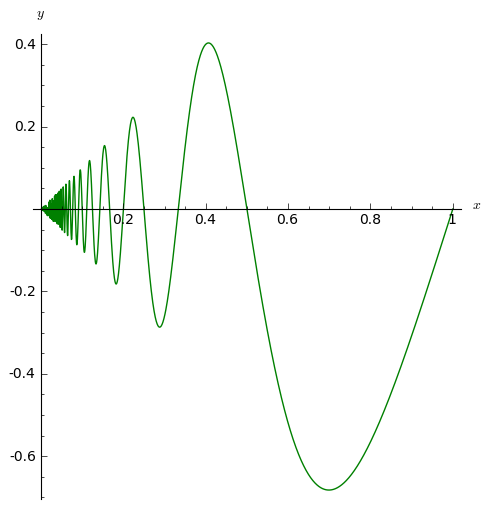
\includegraphics[width=0.48\textwidth]{picturebook/ch1sec1/ex1-1-11}}
\subfloat[Ex 12: Twisted Cubic, $|t|\leq 2$]{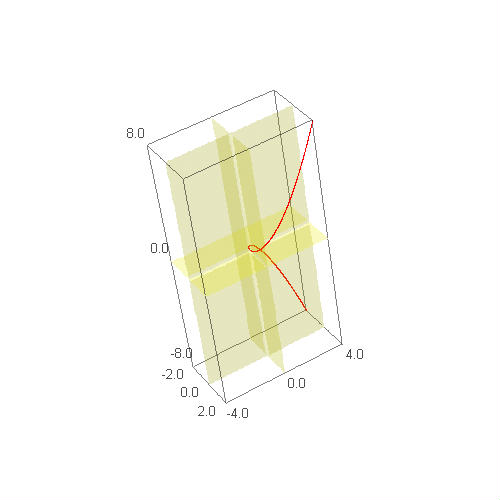
\includegraphics[width=0.48\textwidth]{picturebook/ch1sec1/ex1-1-12a}}
\caption{Curves for Exercises 11 and 12}
\end{figure}

\clearpage

%%%%%%%%%%%%%%%%%%%%%%%%%%%%%%%%%%%%%%%%%%%%%%

\begin{exercise}
Prove that no four distinct points on the twisted cubic lie on a plane.
\end{exercise}

\begin{proof}[Solution]
Recall that the twisted cubic is the space curve
\[
\alpha(t) = (t,t^2, t^3), \qquad t \in \mathbb{R}.
\]
Pick four times $s,t,u,v$ in increasing order. We want to show that $\alpha(v)$ 
does not lie in the plane through $\alpha(s)$, $\alpha(t)$ and $\alpha(u)$. What 
condition might we use to check this?
Well, $\alpha(v)$ lies in this plane exactly when $\alpha(v)-\alpha(s)$ is 
perpendicular to the normal defining the plane. What is the normal? One way to 
find it is to compute with the cross product
\[
\begin{split}
n & = (\alpha(t)-\alpha(s)) \times (\alpha(u)-\alpha(s)) \\
	& = \dots \\
	& = (t-s)(u-s)(u-t) \Big( tu + su + st , (-1)(t + u + s) , 1 \Big) .
\end{split}
\]
So, up to scaling, we may use $n = ( tu + su + st, (-1)(t+u+s), 1) $. Similarly, 
up to scaling,
\[
\alpha(v) - \alpha(s) = (1, v+s , v^2 + vs + s^2 )
\]
We now have that $\alpha(v)$ lies in the plane if and only if
\[
\begin{split}
0 & = n \cdot (\alpha(v) - \alpha(s) ) \\
	& = tu - vt - vu + v^2   = v^2 + (-t-u) v + tu .
\end{split}
\]
This is a quadratic equation for $v$. We apply the quadratic formula to see that 
the roots are $v = u$ and $v= t$. But these have been expressly disallowed since 
our four times are all distinct. Therefore, it is not possible to choose four distinct 
points on the twisted cubic which lie on a plane.
\end{proof}

\clearpage

%%%%%%%%%%%%%%%%%%%%%%%%%%%%%%%%%%%%%%%%%%%%

\begin{exercise}
Consider the ``spiral'' $\alpha(t) = r(t) (\cos(t), \sin(t))$, where $r$ is 
$C^1$ and $0\leq r(t) \leq 1$ for all $t\geq 0$.
\begin{itemize}
\item[a.] Show that if $alpha$ has finite length on $[0,\infty)$ and $r$ is decreasing, 
then $r(t) \rightarrow 0$ as $t \rightarrow 0$.
\item[b.] Show that if $r(t) = 1/(t+1)$, then $\alpha$ has infinite length on $[0,\infty)$.
\item[c.] If $r(t) = 1/(t+1)^2$, does $\alpha$ have finite length on $[0,\infty)$?
\item[d.] Characterize (in terms of the existence of improper integral(s)) the functions 
$r$ for which $\alpha$ has finite length on $[0,\infty)$.
\item[e.] Use the result of part d to show that the result of part a holds even
without the hypothesis that $r$ be decreasing.
\end{itemize}
\end{exercise}

\begin{proof}[Solution]
First, note that the arclength of such a spiral on an interval $[0,u]$ is given by the integral
\[
\text{length}[0,u] = \int_0^u \sqrt{[r'(t)]^2 + [r(t)]^2\, }\ dt. 
\]

If the function $r(t)$ is decreasing, but bounded below by $0$, it must have some limit,
which is necessarily non-negative. Suppose that this limit is $C>0$. Then we see that
$r(t) \geq C$ for all $t$ and 
\[
\text{length}[0,u] = \int_0^u \sqrt{[r'(t)]^2 + [r(t)]^2\, }\ dt \geq \int_0^u C\ dt = Cu .
\]
So we cannot have both that the spiral has finite length and and $r$ decreases to a
\emph{positive} limit. If the spiral has finite length and $r$ decreases, it must
have limit $0$ as $t$ increases without bound.

To deal with the examples, we can compute directly. If $r(t) = \frac{1}{t+1}$, then 
$r'(t) = \frac{-1}{(t+1)^2}$, and
\[
\text{length}[0,u] = \int_0^u \dfrac{1}{1+t}\sqrt{\dfrac{1}{(t+1)^2} +1\,}\ dt.
\]
Since the quantity in the square root is always at least $1$, the integrand here is always
at least $\frac{1}{t+1}$, and we learn that 
\[
\text{length}[0,u] \geq \int_0^u \dfrac{1}{1+t}\ dt = \log u, 
\]
which is unbounded on the interval $(0,\infty)$. So this example has infinite length.


But the example $r(t) = \frac{1}{(t+1)^2}$ works out differently. Here, some work shows
\[
\text{length}[0,u] = \int_0^u \dfrac{1}{(1+t)^2}\sqrt{\dfrac{4}{(t+1)^2} +1\,}\ dt.
\]
In this case, we see that the quantity under the radical is always less than $5$, so
\[
\text{length}[0,u] \leq \sqrt{5}\int_0^u \dfrac{1}{(1+t)^2}\ dt = 
\sqrt{5}\left( 1 - \dfrac{1}{1+u}\right) \leq \sqrt{5}
\]
for any value of $u$. Thus, this spiral curve has finite length.

At this point, it should be clear that our spiral curve will have finite total length
exactly when the improper integral 
\[
\int_0^\infty \sqrt{[r'(t)]^2 + [r(t)]^2\, }\ dt
\]
exists and is finite. Of course, for this improper integral to converge, it is
necessary that the integrand have a limit of zero as $t$ increases without bound.
Note that the quantity under the radical is a sum of squares, which are non-negative.
This means that we cannot have any balancing or cancellation as part of this 
limit, and we must have that each of $r(t)$ and $r'(t)$ limit on $0$ as $t$ increases 
without bound. So the assumption that $r$ is decreasing is not actually necessary.

\end{proof}

\clearpage
%%%%%%%%%%%%%%%%%%%%%%%%%%%%%%%%%%%%%%%%%%%%

\begin{exercise}
Suppose that $\alpha:[a,b]\rightarrow \mathbb{R}^2$ is a smooth parametrized plane curve 
(perhaps not arclength-parametrized). Prove that if the chord length 
$||\alpha(s) - \alpha(t) ||$ depends only on $|s-t|$, then $\alpha$ must be a (subset of a) 
line or a circle.
\end{exercise}

\begin{proof}[Solution] We begin by using Taylor's Theorem on $\alpha$ 
and $\alpha'$ near a fixed $t$:
\begin{align*}
\alpha(t+h) - \alpha(t) & = \alpha'(t) h + \dfrac{1}{2}\alpha''(t) h^2 + 
 \dfrac{1}{6}\alpha'''(t) h^3  +  \rho_1,  \\
\alpha'(t+h) - \alpha'(t) & = \alpha''(t) h + \dfrac{1}{2}\alpha'''(t) h^2 + \rho_2,
\end{align*}
where $\rho_1$ and $\rho_2$ are quantities that satisfy
\[
\lim_{h\rightarrow 0} \dfrac{\rho_1}{h^3} = \lim_{h\rightarrow 0} \dfrac{\rho_2}{h^2} = 0.
\]
These are valid for all sufficiently small $h$ as long as $\alpha$ is $\mathcal{C}^3$, say.
By assumption, we now have that
\[
\begin{split}
0  & = \dfrac{\partial}{\partial t}\left|\left| \alpha(t+h) -\alpha(t) \right|\right|^2 \\
	& = 2\left( \alpha(t+h) - \alpha(t) \right) \cdot \left( \alpha'(t+h) - \alpha'(t) \right) \\
	& = 2\left( \alpha'(t) h + \dfrac{1}{2}\alpha''(t) h^2 + \rho_1 \right) 
	\cdot \left( \alpha''(t) h + \dfrac{1}{2}\alpha'''(t) h^2 + \rho_2 \right) \\
	& = 2(\alpha'(t)\cdot \alpha''(t) ) h^2 + ( \alpha''(t)\cdot \alpha''(t) + \alpha'(t) 
	\cdot \alpha'''(t) ) h^3 + \sigma_1,
\end{split}
\]
where $\sigma_1$ is a function that decays at least as fast as $h^4$ as $h\rightarrow 0$.

Since this holds for all $h$ sufficiently small, we can first divide by $h^2$ and then take
the limit as $h$ goes to zero to
deduce that 
\begin{equation}\label{eq:14-1}
\alpha' \cdot \alpha'' = 0  \quad \text{for all $t$}. 
\end{equation} 
With that in hand, we can then divide through by $h^3$ and take a limit as $h$ goes to zero
to learn that 
\begin{equation}\label{eq:14-2}
\alpha'\cdot \alpha''' +\alpha'' \cdot \alpha''=0 \quad \text{for all $t$}.
\end{equation}
Equation (\ref{eq:14-1}) means that $\alpha'$ and $\alpha''$ are always orthogonal. 
Also since $\frac{d}{dt}(\alpha'\cdot\alpha') = 2\alpha'\cdot\alpha''=0$, 
we get that $||\alpha'||$ is a constant. Thus, $\alpha$ is a constant speed 
parametrized curve.\\

Our next goal is to show that $||\alpha''||$ is constant. This will take 
a little more work, so be prepared. Using the Taylor
approximation for $\alpha$ directly, we have
\[
\begin{split}
||\alpha(t+h) &-\alpha(t)||^2  = (\alpha(t+h)-\alpha(t)) \cdot (\alpha(t+h)-\alpha(t)) \\
 & = (\alpha'(t) h + \dfrac{1}{2}\alpha''(t) h^2 + 
   \dfrac{1}{6}\alpha'''(t) h^3 + \rho_1)
   \cdot(\alpha'(t) h + \dfrac{1}{2}\alpha''(t) h^2 + 
   \dfrac{1}{6}\alpha'''(t) h^3 + \rho_1)\\
& = \alpha'(t)\cdot \alpha'(t) h^2 + \alpha'(t)\cdot\alpha''(t) h^3 +
   \left( \dfrac{1}{3} \alpha'(t)\cdot\alpha'''(t) + 
   \dfrac{1}{4}\alpha''(t)\cdot \alpha''(t) \right) h^4 + \sigma_2
\end{split}
\]
By Equation (\ref{eq:14-1}), the $h^3$ term vanishes. 
We can also use Equation (\ref{eq:14-2}) to simplify the $h^4$ term. Doing so, we
get
\[
||\alpha(t+h) -\alpha(t)||^2 = \alpha'(t)\cdot \alpha'(t) h^2 
  -\dfrac{1}{12}\alpha''(t)\cdot\alpha''(t) h^4 + \sigma_2
\]
Now we are ready! By hypothesis, this quantity does not depend upon $t$, but only on $h$.
So if we fix a value of $h$ and take a derivative with respect to $t$, we get
\[
\begin{split}
0  & = \dfrac{\partial}{\partial t}\left|\left| \alpha(t+h) -\alpha(t) \right|\right|^2 \\
  & = 2\alpha'(t)\cdot \alpha''(t) h^2 - \dfrac{1}{6}\alpha''(t)\cdot\alpha'''(t)h^4 + \sigma_3
\end{split}
\]
Recall that we already know the first term on the right vanishes by Equation (\ref{eq:14-1}).
And if we argue as above, we can deduce that $\alpha'' \cdot \alpha'''$ vanishes for all
values of $t$. That is half the derivative of $||\alpha''(t)||^2$. 
Therefore, $||\alpha''||$ is constant.\\

Note that if $||\alpha''|| = 0$, then $\alpha''=0$ everywhere, so $\alpha'$ is constant. 
This implies that $\alpha$ is a line: $\alpha(t) = v+ t w$.

So, suppose that $||\alpha''||\neq 0$. Since $\alpha'' \neq 0$, we deduce that 
$\{ \alpha'(t), \alpha''(t) \}$ is always a basis of the plane.
By Equation (\ref{eq:14-2}) from the first derivation above, we can write the next constant 
two ways:
\[
z = \dfrac{\alpha'\cdot \alpha'}{\alpha''\cdot\alpha''} = - \dfrac{\alpha'\cdot \alpha'}
{\alpha' \cdot \alpha'''} .
\]
Now consider the point $P$ defined by $ P = \alpha(t) + z \alpha''(t)$. We shall now check 
that this is indeed a point, that is, $P$ does not move.
We compute that the dot product of $P'= \alpha' + z \alpha'''$ with each of our basis vectors is
\begin{align*}
P' \cdot \alpha'& = \alpha' \cdot \alpha' + z \alpha' \cdot \alpha''' = \alpha' \cdot \alpha' 
+ \left( - \dfrac{\alpha'\cdot \alpha'}{\alpha' \cdot \alpha'''} \right) 
\alpha' \cdot \alpha''' = 0 \\
P' \cdot \alpha'' &  = \alpha' \cdot \alpha'' + z \alpha'''\cdot \alpha'' = 0
\end{align*}
So $P'$ is orthogonal to both of our basis vectors, which means $P'=0$.
This means that $P$ is stationary, hence really is a point. Now, we clearly have that 
$||\alpha(t) - P ||^2 = z^2 \alpha'' \cdot \alpha'' $ is a constant. That means, of course, 
that $\alpha$ lies on a circle about $P$.
\end{proof}


\vfill

\end{document}
